\documentclass{article}
\usepackage{graphicx}
\usepackage[utf8]{inputenc}
\usepackage{listings}
\usepackage{color}
\usepackage{amsfonts}
\usepackage{tabularx}
\usepackage{mathtools}
\usepackage[ngerman]{babel}
\newcommand\norm[1]{\left\lVert#1\right\rVert}

\begin{document}
\begin{titlepage}
\centering
    \begin{figure}
    \centering
	    
\includegraphics[width=90mm]{logo_lmu.jpg}
    \end{figure}
	{\scshape\LARGE Ludwig-Maximilians Universität \par}
	\vspace{1cm}
	{\scshape\Large Skript \par}
	\vspace{1.5cm}
	{\huge\bfseries Betriebssysteme\par}
	\vspace{2cm}
	{\Large\itshape Andreas Götzfried\par}
    \vfill
	    basierend auf\par
	    Prof. Dr. C.\textsc{Linnhoff-Popien}
    \vfill
	{\large \today\par}
\end{titlepage}
\tableofcontents{}

\newpage
\section{Einführung}
\subsection{Das Betriebssystem}
\subsubsection{Einordnung der Maschinensprache}
    \begin{figure}[h]
        \centering
	    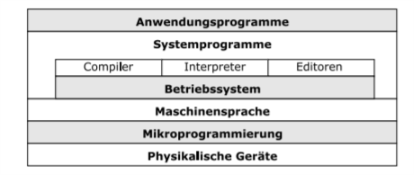
\includegraphics[width=90mm]{Skizzen/1. Kapitel/Hierarchie-der-Funktionen .png}
    \end{figure}
\subsubsection{Aufgaben des Betriebssystems}
    Ein Betriebssystem soll die Komplexität der Maschinensprache mindern. Das Betriebssystem ist eine \textbf{erweiterte Maschine}, die leichter zu programmieren ist als die darunter liegenden Schichten. Außerdem gilt es als \textbf{Ressourcenmanager}, indem es die vorhandenen Systemressourcen (Speicher, CPU, ...) verwaltet und zwischen den Anforderungen der Programme und diesen Ressourcen vermittelt. Für das \textbf{Multiplexing}, das Verteilen von Ressourcen auf mehrere Programme beziehungsweise Nutzer, kann ein \textbf{Time Multiplexing} gewählt werden, das die Ressourcen zeitlich verzahnt vollständig einem Programm zur Verfügung stellt (Prozessor), oder das \textbf{Space Multiplexing}, bei welchem sich mehrere Programme gleichzeitig die Ressourcen teilen (Hauptspeicher). Auch dient das Betriebssystem als \textbf{Kontrollinstanz} für jegliche Zugriffe und unterbindet unerlaubte Zugriffe.\newline
    \textbf{Bestandteile:}\newline
    Ein Betriebssystem besteht aus verschiedenen Programmen, die im Systemmodus(Kernel Mode) priorisiert laufen. Dazu zählen Gerätetreiber, Prozessmanager, Festermanager und andere.\newline
    \textbf{Systemaufrufe:}\newline
    Die Schnittstelle zwischen Anwendungsprogrammen und Betriebssystem wird durch Systemaufrufe definiert. 
\subsubsection{Geschichte der Betriebssysteme}
    \textbf{1. Generation: 1945 bis 1955 (Röhren und Klinkenfelder}\newline
    John von Neumann und Konrad Zuse waren Größen dieser Zeit, die riesige Apparate mit zehntausenden von Röhren und Taktzeiten in Sekunden als erste Rechner herstellten. Programme wurden über Klinkenfelder, später durch Lochkarten ersetzt, gesteckt oder in Maschinencode eingegeben. Programmiersprachen, Assemblersprachen und Betriebssysteme waren unbekannt.\newline
    \textbf{2. Generation: 1955 bis 1965 (Transistoren und Stapelsysteme}\newline
    Die Zuverlässigkeit von Systemen (Mainframe) wurde durch Transistoren erhöht, waren aber extrem teuer. Große Leerlaufzeiten durch die Programme, die durch Lochkarten eingegeben wurden und bis zum Ende durchlaufen mussten, entstanden. Deshalb wurde das Stapelverarbeitungssystem (Batchsystem) eingeführt, welches Aufträge sammelt und vom Mainframe eingelesen wurde. Ein Programmstapel begann mit einer \$JOB Karte, die die maximale Laufzeit, die Abrechnungsnummer und Name des Programmierer übertrug, dann folgte die \$FORTRAN Karte, die das Betriebssystem beauftragte, den Fortran Compiler zu laden, danach das zu übersetzende Programm und eine \$LOAD Karte, die das Programm lud, die \$RUN Karte veranlasste das Betriebssystem, das Programm zu bearbeiten, und mit der \$END Karte wurde die Programmbearbeitung beendet.\newline
    Erste Betriebssysteme waren FMS (Fortran Monitor System) und das IBSYS (IBM Betriebssystem). Diese Betriebssysteme unterbrachen bei jeder I/O-Aktion die CPU.\newline
    \textbf{3. Generation: 1965 bis 1980 (Integrierte Bauelemente und Multiprogramming}\newline
    Diese Generation verwendete integrierte Bauteile. Die Fortschritte waren das \textbf{Spooling}, das Jobs auf Vorrat einlesen und auf Festplatten speichern konnte, und der \textbf{Mehrprogrammbetrieb}, der Space Multiplexing verwendete.\newline
    Da man keinen Zugriff auf das Programm hatte, war ein Dialogbetrieb nötig, deshalb wurde das \textbf{Timesharing}-System (CTSS) entwickelt, welches jedem Benutzer über ein Terminal auf den Rechner zugreifen ließ. Dann wurde \textbf{MULTICS} (Multiplexed Information und Computing Service), ein Timesharing-System, das nur bei Bedarf die Kapazität nimmt, die es benötigt. Eine Einbenutzerversion \textbf{UNICS} (Uniplexed Information und Computing System) später \textbf{UNIX} (in C programmiert) wurde später vorgestellt.\newline
    \textbf{4. Generation: seit 1980 (PCs)}\newline
    Die Entwicklung von LSI (Large Scale Integration) Schaltkreisen erhöhte die Rechenleistung. Betriebssysteme waren \textbf{MS-DOS} (Microsoft Disk Operation System) und UNIX. zusätzlich wurde die \textbf{GUI} (Graphical User Interface) erfunden.\newline
    Betriebssysteme für Rechner lassen sich nun unterteilen:
    \begin{itemize}
        \item Netzwerk-Betriebssystem: Der Benutzer kennt mehrere Rechner mit eigenem Betriebssystem und kann sich gezielt auf diesen anmelden
        \item Verteiltes Betriebssystem: Soll wie ein Einprozessorsystem erscheinen, damit die Nutzer nicht wissen, wo Programme ablaufen und Daten liegen
    \end{itemize}
    \textbf{5. Generation: seit circa 2000 (mobile Betriebssysteme)}\newline
    Erstes Smartphone ist der Simon Personal Computer von IBM und BellSouth. Ab den iPhones wurde der Touch Screen populär. Anforderungen waren energiesparender und effizienter Zugriff wegen den begrenzten Ressourcen. Android basiert auf stark angepasstem Linux-Kernel mit besonders ressourcenschonender Programmierung. Die Sicherheit wird über eine Distributionskanal des Betriebssystems gewährleistet (PlayStore).
\subsubsection{Arten von Betriebssystemen}
    \begin{itemize}
        \item Mainframe-Betriebssystem: Optimiert auf gleichzeitig ablaufende Prozesse mit vielen I/O-Operationen
        \item Server-Betriebssystem: Kleine Webserver und Workstations
        \item Multiprozessor-Betriebssystem: Bei mehreren Prozessoren wird ein spezielles Betriebssystem benötigt, das die Verteilung der Aufgaben an die Prozessoren übernimmt
        \item PC-Betriebssystem: Generische Plattform für viele Anwendungen und Anforderungen
        \item Echtzeit-Betriebssystem: Steuerung von Maschinen. Weiches oder hartes System, bei geringer oder größerer Toleranz bei I/O-Operationen
        \item Embedded Betriebssystem: Für PDAs und mobile Endgeräte entwickelt; Kommunikationsschnittstellen sind wichtig
        \item Betriebssystem für Chipkarten: Mini-Betriebssystem, z.B. im Zusammenhang mit RFID-Technologie
    \end{itemize}
    
\newpage
\section{Prozesse}
\subsection{Programme und Unterprogramme}
\subsubsection{Vom Programm zum Maschinenprogramm}
    Ein zur Ausführung befindliches Programm ist ein Folge von Befehlen, die vom Prozessor ausgeführt werden. Um eine höhere Programmiersprache in Maschinenprogramm zu übersetzen, wird ein Compiler benötigt. Soll das Maschinenprogramm ausgeführt werden, bekommt er einen Speicherbereich zugewiesen mit genau so viel Speicherzellen wie Befehle im Programm, in welchen dann die Befehle kopiert werden.  
\subsubsection{Unterprogramme und Prozeduren}
    \textbf{Offenes Unterprogramm:}\newline
    Der Programmtext wird in das Hauptprogramm kopiert. Probleme beim Ändern des Unterprogramms und bei langen Unterprogrammen (Speicherplatz).\newline
    \textbf{Geschlossenes Unterprogramm (Prozedur):}\newline
    Das Programm wird über seine Anfangsadresse angesprungen und bei beenden über die Rückkehradresse verlassen. Announcements sind Prozeduren ohne Ergebnisparameter, Invocation mit. Auch rekursive Unterprogramme sind möglich.\newline
    Die Anfangsadresse wird mit dem Befehl CALL direkt angesprungen. RET bewirkt den Rücksprung. Die Prozedur kann Aufrufparameter und Rückgabewerte besitzen.\newline
    Die Informationen werden entweder durch ein Stack ausgetauscht, die eine beliebige Anzahl von Parametern definiert, oder durch spezielle Register, die in der Speicherhierarchie ganz oben stehen und geringste Zugriffszeiten haben.\newline
    \\
    \textbf{2.1.2.1 Die Befehle CALL und RET}\newline
    \begin{lstlisting}
        COMMAND JMP addr
        BEGIN 
            PC := addr;
        END
    \end{lstlisting}
    Der Befehl CALL unterscheidet sich vom Befehl JUMP durch die Sicherung der Rücksprungadresse. Entweder wird diese in einem Register gesichert oder auf einem Stack.
    \begin{lstlisting}
        COMMAND CALL addr
        BEGIN 
            RA := PC + 1 | PUSH (PC + 1);
            PC := addr;
        END
    \end{lstlisting}
    Entsprechend beim RET Befehl.
    \begin{lstlisting}
        COMMAND RET
        BEGIN 
            PC := RA | PC := POP;
        END
    \end{lstlisting}
    \\
    \textbf{2.1.2.2 Schema für Unterprogrammaufrufe}\newline
    Eine \textbf{Nested Procedure} ruft in ihrem eigenen Programm ein weiteres Unterprogramm auf, wobei immer wieder die RET-Adresse auf das aufrufende Programm weitergegeben werden muss.  
    \\
    \textbf{2.1.2.3 Module}\newline
    Module sind zum Beispiel Unterprogramme, Komponenten des Betriebssystems, Benutzerprogramme oder Prozesse. Zu einem Zeitpunkt kann nur ein Modul einem Rechnerkern zugeordnet werden. Die Zustände von Modulen, den Rechnerkernzustand, Speicherabbildungstabellen, Programmcode und Daten, müssen verwaltet werden. Eine Aktivierung eines Moduls kann durch einen Unterprogramm-/Prozeduraufruf, einem Systemaufruf oder einem Prozesswechsel erreicht werden.\newline
    \textbf{Server und Client:}\newline
    In verteilten Systemen stellen Module auch über Rechnergrenzen hinweg Dienste bereit.\newline
    \textbf{Dienst;}\newline
    Ein Dienst ist eine Funktion, die von einem Objekt an einer Schnittstelle angeboten wird.\newline
    \textbf{Entfernte Prozeduraufrufe:}\newline
    Da sich zwei Computer nicht den gleichen Speicher teilen, benötigt man entfernte Prozeduraufrufe, um Module aufrufen zu können.
\subsubsection{Realisierung eines Unterprogrammaufrufs}
    Die Modell-Maschine MI verfügt über die Register PC (Programmzähler), SP (Stack-Pointer) und R0 bis R14, wobei R12/R13 nicht frei genutzt werden dürfen, sondern die Ablageadresse des ersten Aufrufparameters und die Basisadresse des lokalen Datenraums des Unterprogramms erhalten. Außerdem besitzt die MI noch einen Kellerspeicher mit ausreichendem Speicherplatz. Die Adressen der Kellerzellen werden bei wachsendem Keller kleiner. Alle Speicherzellen sind 4 Bytes breit und können damit alle Maschinenbefehle zu 32-Bit-Wörtern kodiert.\newline
    Die Parameter des Unterprogrammaufrufs werden in umgekehrter Reihenfolge auf den Keller gelegt (lokaler Datenraum) und der Rückgabewert bekommt ebenfalls einen Kellerplatz. Die Register der Maschine MI sind Callee-saved, dass heißt das aufgerufene Unterprogramm trägt die Verantwortung dafür, dass der Kontext des Aufrufers nach dem Rücksprung unverändert dem Kontext vor dem Unterprogrammaufruf entspricht.\newline
    Befehle der MI sind:
    \begin{itemize}
        \item PUSH val: Legt Wert auf den Keller
        \item PUSH reg: Legt Inhalt des Registers auf Keller
        \item PUSHR: Sichert gesamen CPU-Register-Kontext (R0 bis R14)
        \item POP reg: Legt Inhalt der obersten Kellerzelle in Register
        \item POPR: Stellt gesamten Register-Kontext her
        \item MOVE addr, reg: Kopiert Adresse ins Register
        \item MOVE reg1, reg2: Kopiert Inhalt von Register 1 ins Register 2
        \item CALL addr: Sprung zu Adresse und Sicherung der Rücksprungadresse auf Keller
        \item RET: Rücksprung zum Aufrufer
    \end{itemize}
    Parameter können vom Hauptprogramm an das Unterprogramm und umgekehrt auf die Art Call by value (Wertübergabe) oder Call by referenz (Adressübergabe).
\subsubsection{Rekursive Prozeduraufrufe}
    Zu beachten ist hierbei, dass im i-ten Unterprogramm das Ergebnis in den lokalen Datenraum des (i-1)-ten Unterprogramms geschrieben wird. Daher ist es so wichtig, erst Speicherplatz für ein Ergebnis einzurichten und dann zu springen.
\subsection{Prozesse}
\subsubsection{Das Prozess-Konzept}
    \textbf{2.2.1.1 Grundlagen von Prozessen}\newline
    Im Vergleich zu Berechnungen durch den Prozess sind Operationen auf E/A-Geräten oft erheblich langsamer. Es soll verhindert werden, dass die CPU beim Warten auf das Ende von E/A-Operationen still steht.\newline
    Ein \textbf{Prozess} ist ein in Ausführung befindliches Maschinenprogramm mit aktuellem Wert des Programmzählers und den aktuellen Werten der Register und der Variablen.\newline
    Zum \textbf{Prozesskontext} gehören alle Informationen, die den aktuellen Ausführungszustand eines Prozessen genau beschreiben. Dazu zählt die CPU-Register-Belegungen und die Prozess-Status-Informationen. Hiermit lässt sich ein unterbrochener Prozess wieder fortsetzen.\newline
    Als \textbf{Image} eines Prozesses bezeichnet man die Gesamtheit der physischen Bestandteile eines Prozesses, also die Befehlsfolge und Kontext mit lokalen und globalen Variablen und Ausführungsstack. Hiermit lässt sich ein Prozess auf einem anderen Computer fortsetzen.\newline
    Beim \textbf{Uniprogramming} werden Prozesse sequenziell nacheinander, vollständig und ohne Unterbrechung ausgeführt.\newline
    Beim \textbf{Multiprogramming} wird zwischen mehreren Prozessen pseudo-parallel hin- und hergeschalten.\newline
    Beim \textbf{Multiprocessoring} stehen mehrere Prozessoren zur Verfügung, damit Prozesse echt-parallel ausgeführt werden können.\newline
    \\
    \textbf{2.2.1.2 Erzeugung von Prozessen}\newline
    Mit \textit{fork} wird eine identische Kopie (Kindprozess) des Prozesses unter Unix erzeugt. Unter MS DOS können Vater- und Kindprozesse nicht parallel ausgeführt werden. Hier wird der Vaterprozess suspendiert bis der Kindprozess fertig ist.\newline
    Durch \textbf{Dispatching} wird ein Rechnerkern an einen Prozess zugeordnet.\newline
    Die Ursachen für die Erzeugung eines Prozesses sind neue Stapelaufträge, die Benutzeranmeldung, ein Dienstleistungsprozess oder Kindprozesse.\newline
    In Unix sind alle Prozesse Nachkommen des \textit{init}-Prozesses.\newline
    Um einen Prozess zu erzeugen muss zuerst der Prozess einen Identifikator zugewiesen bekommen und mit dieser PID in die Prozesstabelle eingetragen. Dem Prozess wird dann Speicherplatz für das Prozess-Image zugeordnet. Danach wird der Prozesskontrollblock (PCB) initialisiert, die erforderlichen Links gesetzt und in eine Liste eingefügt werden (Ready bz. Ready, Suspend). Gegebenenfalls sind Datenstrukturen zu erweitern.\newline
    \\
    \textbf{2.2.1.3 Realisierung von Multiprogramming}\newline
    Aus Sicht des Prozessors ist es egal, welchen Code er ausführt und für ein Programm ist es nur wichtig, dass die Reihenfolge der Befehle eingehalten wird. Der \textbf{Dispatcher} ist ein Prozess, der einen Prozess unterbrechen und einem anderen Prozess dem Prozessor zuordnen kann.\newline
    \\
    \textbf{2.2.1.4 Das 2-Zustands-Prozessmodell}\newline
    Mit \textbf{Running} und \textbf{Not running} wird dieses einfache Prozessmodell beschrieben.
    \begin{figure}[h]
        \centering
	    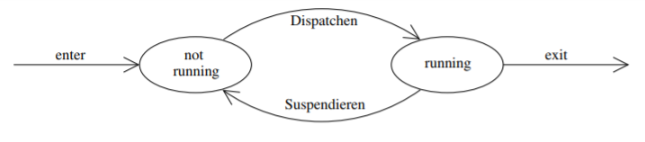
\includegraphics[width=90mm]{Skizzen/2. Kapitel/2-Zustandsmodell.png}
    \end{figure}
    Zwei Anforderungen an Information müssen abgeleitet werden können. Der aktuelle Zustand des Prozess muss beschreibbar sein und die Speicherinformationen des Prozesses müssen abrufbar sein.\newline
    Der \textbf{Scheduler} setzt die Strategie um, nach der entschieden wird, wann welcher Prozess als nächstes rechnen darf. Der \textbf{Dispatcher} übernimmt das Suspendieren und die Zuweisung der CPU an einen Prozess.\newline
    \\
    \textbf{2.2.1.5 Das 5-Zustands-Prozessmodell}\newline
    Hier kommen Ready, Blocked, New und Exit dazu und Not running ist überflüssig.
    \begin{figure}[h]
        \centering
	    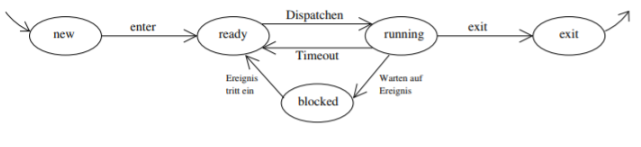
\includegraphics[width=90mm]{Skizzen/2. Kapitel/5-Zustandsmodell.png}
    \end{figure}
    Die Blocked Queue kann auch noch in priorisierte Queue eingeteilt werden.\newline
    \\
    \textbf{2.2.1.6 Das 7-Zustands-Prozessmodell}\newline
    Wenn der Hauptspeicher alle Prozesse in die Blocked Queue schiebt, steht kein Speicherplatz für weitere Prozesse zur Verfügung. Dieses Problem kann durch größeren Hauptspeicher oder Swapping gelöst werden.\newline
    \textbf{Swapping} lagert Teile eines blockierten Prozesses auf die Platte aus.\newline
    Der \textbf{Virtuelle Speicher} ist die Menge an Speicher, die dem Betriebssystem maximal zur Abbildung von Prozessen auf dem Hintergrundspeicher zur Verfügung stehen.\newline
    Das Swapping kann auch schon im 5-Zustands-Modell eingeführt werden.
    \begin{figure}[h]
        \centering
	    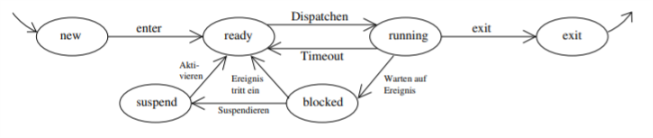
\includegraphics[width=90mm]{Skizzen/2. Kapitel/5-Zustandsmodell-mit-Suspend.png}
    \end{figure}
    Wenn man bei diesem Modell sowohl bei den im Hauptspeicher enthaltenen als auch bei den ausgelagerten Prozessen zwischen blockierten und nicht blockierten unterscheidet, entsteht das 7-Zustands-Modell.
    \begin{figure}[h]
        \centering
	    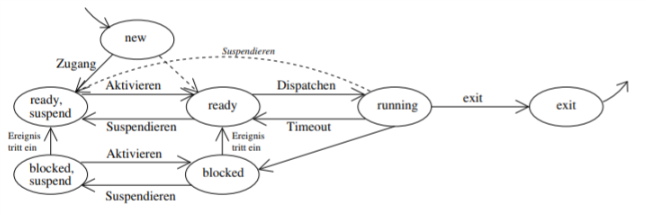
\includegraphics[width=90mm]{Skizzen/2. Kapitel/7-Zustandsmodell.png}
    \end{figure}
\subsubsection{Prozessbeschreibung}
    \begin{figure}[h]
        \centering
	    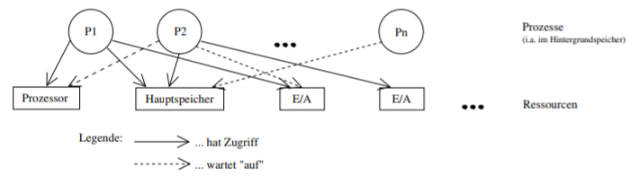
\includegraphics[width=90mm]{Skizzen/3. Kapitel/Systemressourcen.png}
    \end{figure}
    \textbf{2.2.2.1 Kontrollstrukturen des Betriebssystems}\newline
    Die \textbf{Seitenrahmen (Frames)} beschreiben die Einteilung des Hauptspeichers in Speicherzellblöcken. Auch wird die Instruktionsfolge eines Prozesses in \textbf{Seiten} aufgeteilt.\newline
    Die \textbf{Speichertabellen} dienen dazu, den Überblick über den Haupt- und virtuellen Speicher zu behalten, wobei gleich ein Teil des Hauptspeichers für das Betriebssystem reserviert ist. Sie sind aufgebaut mit der Zuordnung der Seiten eines Prozesses zu den Frames, aus der Zuteilung des virtuellen Speichers zu den Prozessen und den Schutzattributen von Seiten und Frames.\newline
    Die \textbf{E/A-Tabellen} dienen zur Verwaltung der E/A-Geräte. Sie sind entweder vverfügbar oder einem Prozess zugeordnet, wobei hier das Betriebssystem den Status des Geräts kennt.\newline
    Die \textbf{Dateitabellen} enthalten Informationen über die Existenz von Dateien, über ihren Ort im Hintergrundspeicher, Status und Attributen. Falls seperates Dateisystem existiert, so kann ein Großteil dieser Informationen darin enthalten sein.\newline
    Die \textbf{Prozesstabellen} enthalten Informationen zur Verwaltung aller Prozesse.\newline
    \\
    \textbf{2.2.2.2 Prozesskontrollstrukturen}\newline
    Das Betriebssystem muss wissen, wo der Prozess gespeichert ist und welche Werte die relevanten Attribute besitzen.\newline
    Der Prozess kann lokalisiert werden, indem man die \textbf{dynamische Partitionierung (Segmentierung)} einsetzt, welche den Prozess als zusammenhängenden Block in den Speicherzellen ablegt, einen Teil dieser Daten in den Hauptspeicher geladen wird und bei Ausführung alles in den gesamten Prozess in den Hauptspeicher legt. Anders kann es bei einer \textbf{festen Partitionierung (Paging)} ablaufen. Hier wird der Speicher in feste Blöcke partitioniert und ein Prozess-Image in aneinander grenzenden Blöcken gespeichert. Der gesamte Prozess-Image befindet sich hierbei im Hintergrundspeicher und falls ein Teil benötigt wird, wird dieser in freie Frames des Hauptspeichers kopiert.\newline 
    Um die \textbf{Prozessattribute} zu kontollieren wird dies im Prozesskontrollblock (PCB) mit Prozessidentifikation, Prozesszustandsinformation und Prozesskontrollinformation gespeichert. Die \textbf{Prozessidentifikation} enthält den numerischen Identifikator (PID), den Identifikator des Elternprozesses und die ID des Eigentümers. Die \textbf{Prozesszustandsinformationen} beinhalten den Inhalt der Prozessregister und das Programmstatuswort, welches die Menge der Register mit Statusinformationen beschreibt. Die \textbf{Prozesskontrollinformation} besteht aus Scheduling- und Zustandsinformationen wie Prozesszustand, Priorität, Schedling-Strategie und Ereignisse, den Datenstrukturen (z.B. Referenz auf nächsten Prozess), Signalen oder Nachrichten zwischen Prozessen und zusätzlichen Informationen über Privilegien ddes Prozesses, Speichermanagement,  Eigentümerverhältnissen und ähnlichem.\newline
    Die Prozessstruktur im Hintergrundspeicher sieht wie folgt aus.\newline
    \\
    \textbf{2.2.2.3 Zusammenfassung der Verwaltung und Beschreibung von Prozessen}\newline
\subsubsection{Prozesskontrolle}
    \textbf{2.2.3.1 Prozesswechsel (Kontext-Switch)}\newline
    \\
    \textbf{2.2.3.2 Unterbrechungen}\newline
    \\
    \textbf{2.2.3.3 Moduswechsel}\newline
    \\
    \textbf{2.2.3.4 Konflikte bei Unterbrechungen}\newline
    \\
    \textbf{2.2.3.5 Ausführung des Betriebssystems}\newline
\subsection{Threads}
\subsubsection{Multithreading}
\subsubsection{Threadzustände}
\subsubsection{User-Level-Threads (ULT)}
\subsubsection{Kernel-Level-Threads (KLT)}
\subsubsection{Kombinierte Konzepte}
\subsubsection{Andere Formen paralleler Abläufe}
\subsection{Scheduling}
\subsubsection{Das Prinzip des Schedulings}
\subsubsection{Scheduling-Algorithmen}
\subsubsection{Prozesswechsel}
\subsubsection{Arten des Schedulings}

\newpage
\section{Multiprocessing}
\subsection{Deadlocks bei Prozessen}
\subsubsection{Motivation der Deadlocks anhand zweier Beispiele}
\subsubsection{Das Prinzip der Deadlocks}
\subsubsection{Deadlock Prevention}
\subsection{Prozesskoordination}
\subsubsection{Nebenläufigkeit von Prozessen}
\subsubsection{Kritische Bereiche}
\subsubsection{Wechselseitiger Ausschluss}
\subsubsection{Semaphore}
\subsubsection{Monitore}
\subsubsection{Message Passing}

\newpage
\section{Ressourcenverwaltung}
\subsection{Speicher}
\subsubsection{Speicherverwaltung}
\subsubsection{Speicherpartitionierung}
\subsubsection{Virtueller Speicher}
\subsubsection{Paging}
\subsubsection{Segmentierungsstrategien}
\subsection{E/A Verwaltung}
\subsubsection{Klassifizierung von E/A-Geräten}
\subsubsection{E/A Techniken}

\newpage
\section{Interprozesskommunikation}
\subsection{Lokale Interprozesskommunikation}
\subsubsection{Grundlagen des Nachrichtenaustauschs}
\subsubsection{Pipes}
\subsubsection{FIFOs}
\subsubsection{Stream Pipes}
\subsubsection{Sockets}
\subsection{Verteilte Systeme}
\subsubsection{Einführung in Verteilte Systeme}
\subsubsection{Kommunikation in Verteilte Systeme}
\end{document}